\chapter{Foundations}

\section{Tools}

\subsection*{Python}

Python is an interpreted, object-oriented, high-level programming language with dynamic semantics.
The easy-to-learn syntax enables a Rapid Application Development and offers great readability.
Key features are built in data structures, dynamic typing and binding.
\cite{python-lang}
It has its own package manager called "Python Package Index (PyPi)".
The language is compiled at execution.
It is available for all major platforms without charge.
The programming language is open-source and maintained by the Pthon Software Foundation.
\cite{python-software-foundation}


\subsection*{NumPy}

NumPy is a package for Python.
It enables scientific computing with N-dimensional array objects.
Moreover, it supports arithmetic operations of arrays with different shapes, type casting and basic linear algebra functions.
\cite{numpy-package, numpy-broadcasting}


\subsection*{Tensorflow}

Tensorflow is an entire ecosystem for solving problems with machine learning.
It is developed and maintained by the Google Brain team.
In 2015 it was released under the Apache 2.0 open-source license.
It offers multiple levels of abstraction for building, training and testing models.
Visualisations of the code and intuitive debugging allow the developers more flexibility.
Large machine learning training tasks can be done with distributed training on different hardware configurations without changing the model definition.
Trained models can be directly put into production.
Moreover, Tensorflow offers support for multiple languages and platforms.
\cite{tensorflow-about}

\subsubsection*{Core Concepts}

Tensorflow consists of a server client architecture.
The core is located on the server side and is developed in the programming language C++.
Developers use client liberaries in different languages to interact with the core.
The general application programming interfaces (APIs) of Tensorflow are shown in Figure \ref{fig:tensorflow_programming_environment_image}.

\begin{figure}[H]
    \centering
    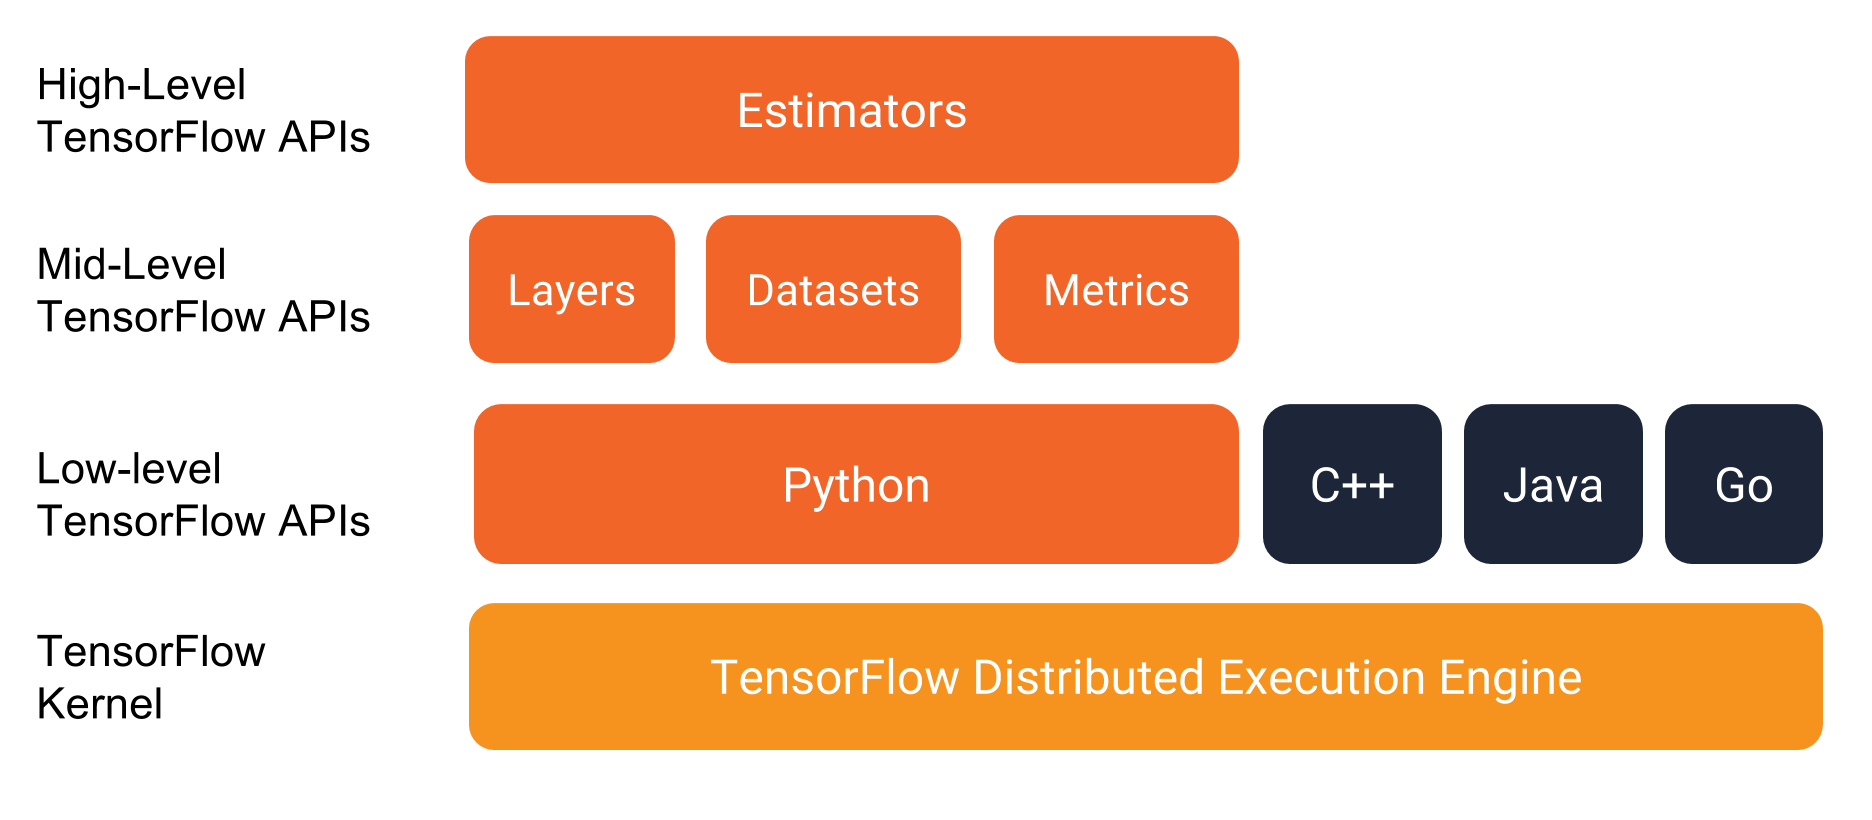
\includegraphics[width=\textwidth]{tensorflow_programming_environment}
    \caption{\cite{tensorflow_programming_environment_image} Tensorflow programming environment}
    \label{fig:tensorflow_programming_environment_image}
\end{figure}

The most important concept for developers is the dataflow graph functionality.
All variables, constants and operations form a computation graph.
Parts of the graph can be started and calculated across a set of local and remote devices.
Figure \ref{fig:tensorflow_graph_image} shows an example of a computation graph:

\begin{figure}[H]
    \centering
    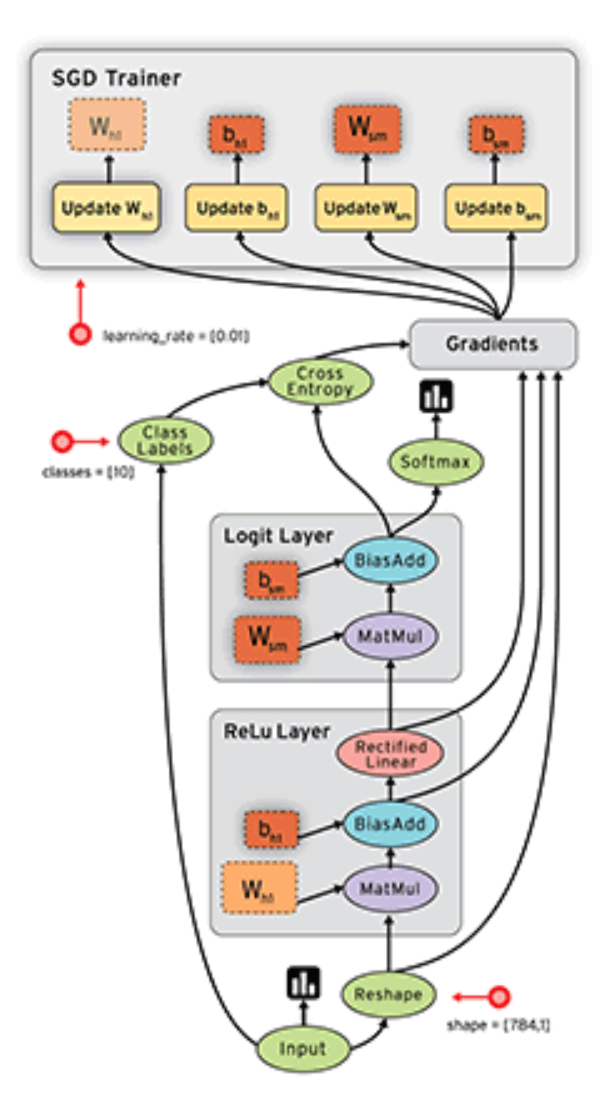
\includegraphics[scale=.5]{tensors_graph}
    \caption{\cite{tensorflow_graph_image} Tensorflow graph}
    \label{fig:tensorflow_graph_image}
\end{figure}

\section{MNIST Dataset}

\begin{figure}[H]
    \centering
    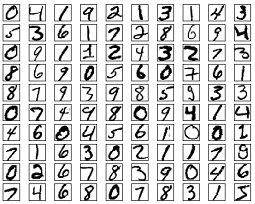
\includegraphics{mnist_100_digits}
    \caption{\cite{mnist_examples_image} Examples of handwritten digits in the mnist dataset}
    \label{fig:mnist_examples}
\end{figure}

The MNIST database is a public available dataset of handwritten digits.
It contains a set of 60,000 training images and 10,000 test images.
The digits are size-normalized and centered photos with a fixed-size of 28 by 28 pixels.
The numbers are created by approximately 250 writers. 
\cite{mnist-database}
The Dataset pertains to one of the most popular datasets for research purposes of new machine learning algorithms.
It is a great resource to test new neural network algorithms in a supervised learning manner.

\section{Deep Neural Network}
\label{foundations_deep_neural_network}

The Introduction provides a general overview of a neural network.
This section shows the construct and the mathematics of the network, that the reimplementation of the Elastic Weight Consolidation uses.

As described, a neural network is a collection of layers.
Every layer contains a fixed number of neurons.
Each neuron is connected to all the neurons on the layer before.
The connections are called weights and each weight holds a value.
\newline
Each neuron computes all the input values (x) with the weights (w) and applies a bias (b) to predict the result (y).
Figure \ref{fig:dnn_node_procedure} shows the computation structure of each neuron in the network.
\cite{math_nn_skalski}

\begin{figure}[H]
    \centering
    \begin{tikzpicture}[
        init/.style={
        draw,
        circle,
        inner sep=2pt,
        font=\Huge,
        join = by -latex
        },
        squa/.style={
        draw,
        inner sep=2pt,
        font=\Large,
        join = by -latex
        },
        start chain=2,node distance=13mm
        ]
        \node[on chain=2] 
        (x2) {$x_2$};
        \node[on chain=2,join=by o-latex] 
        {$w_2$};
        \node[on chain=2,init] (sigma) 
        {$\displaystyle\Sigma$};
        \node[on chain=2,squa,label=above:{\parbox{2cm}{\centering Activation \\ function}}]
        {$f$};
        \node[on chain=2,label=above:Output,join=by -latex] 
        {$y$};
        \begin{scope}[start chain=1]
            \node[on chain=1] at (0,1.5cm) 
            (x1) {$x_1$};
            \node[on chain=1,label=above:Weights,join=by o-latex] 
            (w1) {$w_1$};
        \end{scope}
        \begin{scope}[start chain=3]
            \node[on chain=3] at (0,-1.5cm) 
            (x3) {$x_3$};
            \node[on chain=3,join=by o-latex] 
            (w3) {$w_3$};
        \end{scope}
        \node[label=above:\parbox{2cm}{\centering Bias \\ $b$}] at (sigma|-w1) (b) {};
        
        \draw[-latex] (w1) -- (sigma);
        \draw[-latex] (w3) -- (sigma);
        \draw[o-latex] (b) -- (sigma);
        
        \draw[decorate,decoration={brace,mirror}] (x1.north west) -- node[left=10pt] {Inputs} (x3.south west);
    \end{tikzpicture}
    \caption{\cite{dnn_neuron_basic_overview} Neuron computation structure}
    \label{fig:dnn_node_procedure}
\end{figure}

The output of each neuron is calculated as follows: \cite{medium_nn_from_scratch}

\begin{equation}
y = b + \sum_{i} x_i w_i
\end{equation}

To be able to ensure the quickest calculation possible, vectorisation and matrixes are used.
All Weights coming from the previous layer get stacked to a matrix W together.
The biases on each layer are connected to a vector.
This results in the following calculation
: \cite{medium_nn_from_scratch}

\begin{equation}
X = [ x_1 \dots x_i ]; \space W = 
\begin{bmatrix}
    x_{11} & \dots  & x_{1j} \\
    \vdots & \ddots & \vdots \\
    x_{i1} & \dots  & x_{ij}
\end{bmatrix}; \space
B = [ b_1 \dots b_j ]
\end{equation}

\begin{equation}
    Y = X * W + B
\end{equation}

Finally, the result of this calculation is passed through an activation function.
This activation function is the key element of a neural network.
Without it, a neural network would just be a combination of linear functions, which could be combined into one linear function.
The activation function modifies the result.
Important to mention is, that the activation function has a significant impact on the speed of learning.
The network in this article uses the ReLU as the activation function for all hidden layers \cite{math_nn_skalski,relu}:

\begin{equation}
    ReLU(x) = max(0,x)
\end{equation}

The unnormalized predictions (logits) of the last layer are computed without the activation function.
Still, they are quiet similar to the hidden layer calculations:

$$l = (x*w)+b$$

The softmax function normalizes the logits:

\begin{equation}
    \begin{split}
        S & : \mathbb{R}^K \to \mathbb{R}^K
        \\
        S(x)_i & = \frac{e^{k_i}}{\sum_{k=1}^K e^{x_k}} \: ; i = 1, …, K
    \end{split}
\end{equation}
\begin{equation}
    p = S(l)
\end{equation}

After a prediction the network needs a source of information on the progress of the learning process.
This is where the loss function is introduced.
It is designed to show how bad the classification to the right solution is.
In this article the crossentropy loss function is used.
\cite{math_nn_skalski, medium_nn_from_scratch}

\begin{equation}
    \mathcal{L}^{CE}(p,y) = -\sum_{i=1}^K y_i \log(p_i)
\end{equation}

In the training, the dataset is split into multiple batches.
These batches include a fixed number of samples from the dataset.
The joining of samples enables a much faster prediction process.
This process of calculating a result of the network is called forward propagation.
Within this process, the network calculates a result based on the inputs.
This is happening due to the parameters and functions of the network.
On this output the learning process gets applied.
\cite{math_nn_skalski, medium_nn_from_scratch}
\newline
The learning process is about adapting the weights and biases to optimize the accuracy.
This is done by minimizing the loss function.
The process of updating the weights and biases is called Backpropagation.
It is an algorithm which calculates error gradients with respect to each network variable.
Those gradients are later used in an optimization algorithm called Gradient Descent.
This method searches a function minimum.
After the minimum is found, it applies its results to all parameters in the network.
By adjusting the learning rate of the backpropagation, the developer has the control over the value adjustment.
He defines how detailed each learning step should be.
\cite{math_nn_andrey}
\newline
Iterating the Gradient Descent algorithm several times over different examples will most likely result in a properly trained neural network.

\section{Catastrophic Forgetting}
\label{catastrophic_forgetting}

Catastrophic forgetting happens, when a trained network gets retrained with a new dataset.
This dataset could include completely new classes (disjoint MNIST) or the same classes with new information (permuted MNIST).
The effect is that the network forgets all the information learned in the previous training.
\newline
Figure \ref{fig:catastrophic_forgetting_d91_example} and Figure \ref{fig:catastrophic_forgetting_d55_example} show catastrophic forgetting in action.
The figures demonstrate the training of task $T_1$ (white background) and re-training with task $T_2$ (gray background).
The blue line ($\triangle$) represents the accuracy on $T_1$ and the red line ($\square$) on $T_2$.
\newline
The neural network uses 784 inputs, 3 hidden layer with 800 neurons and 10 output classes.
Each task is trained with a learning rate of 0.001, 2,500 iterations and a batch size of 100.

\begin{figure}[H]
    \centering
    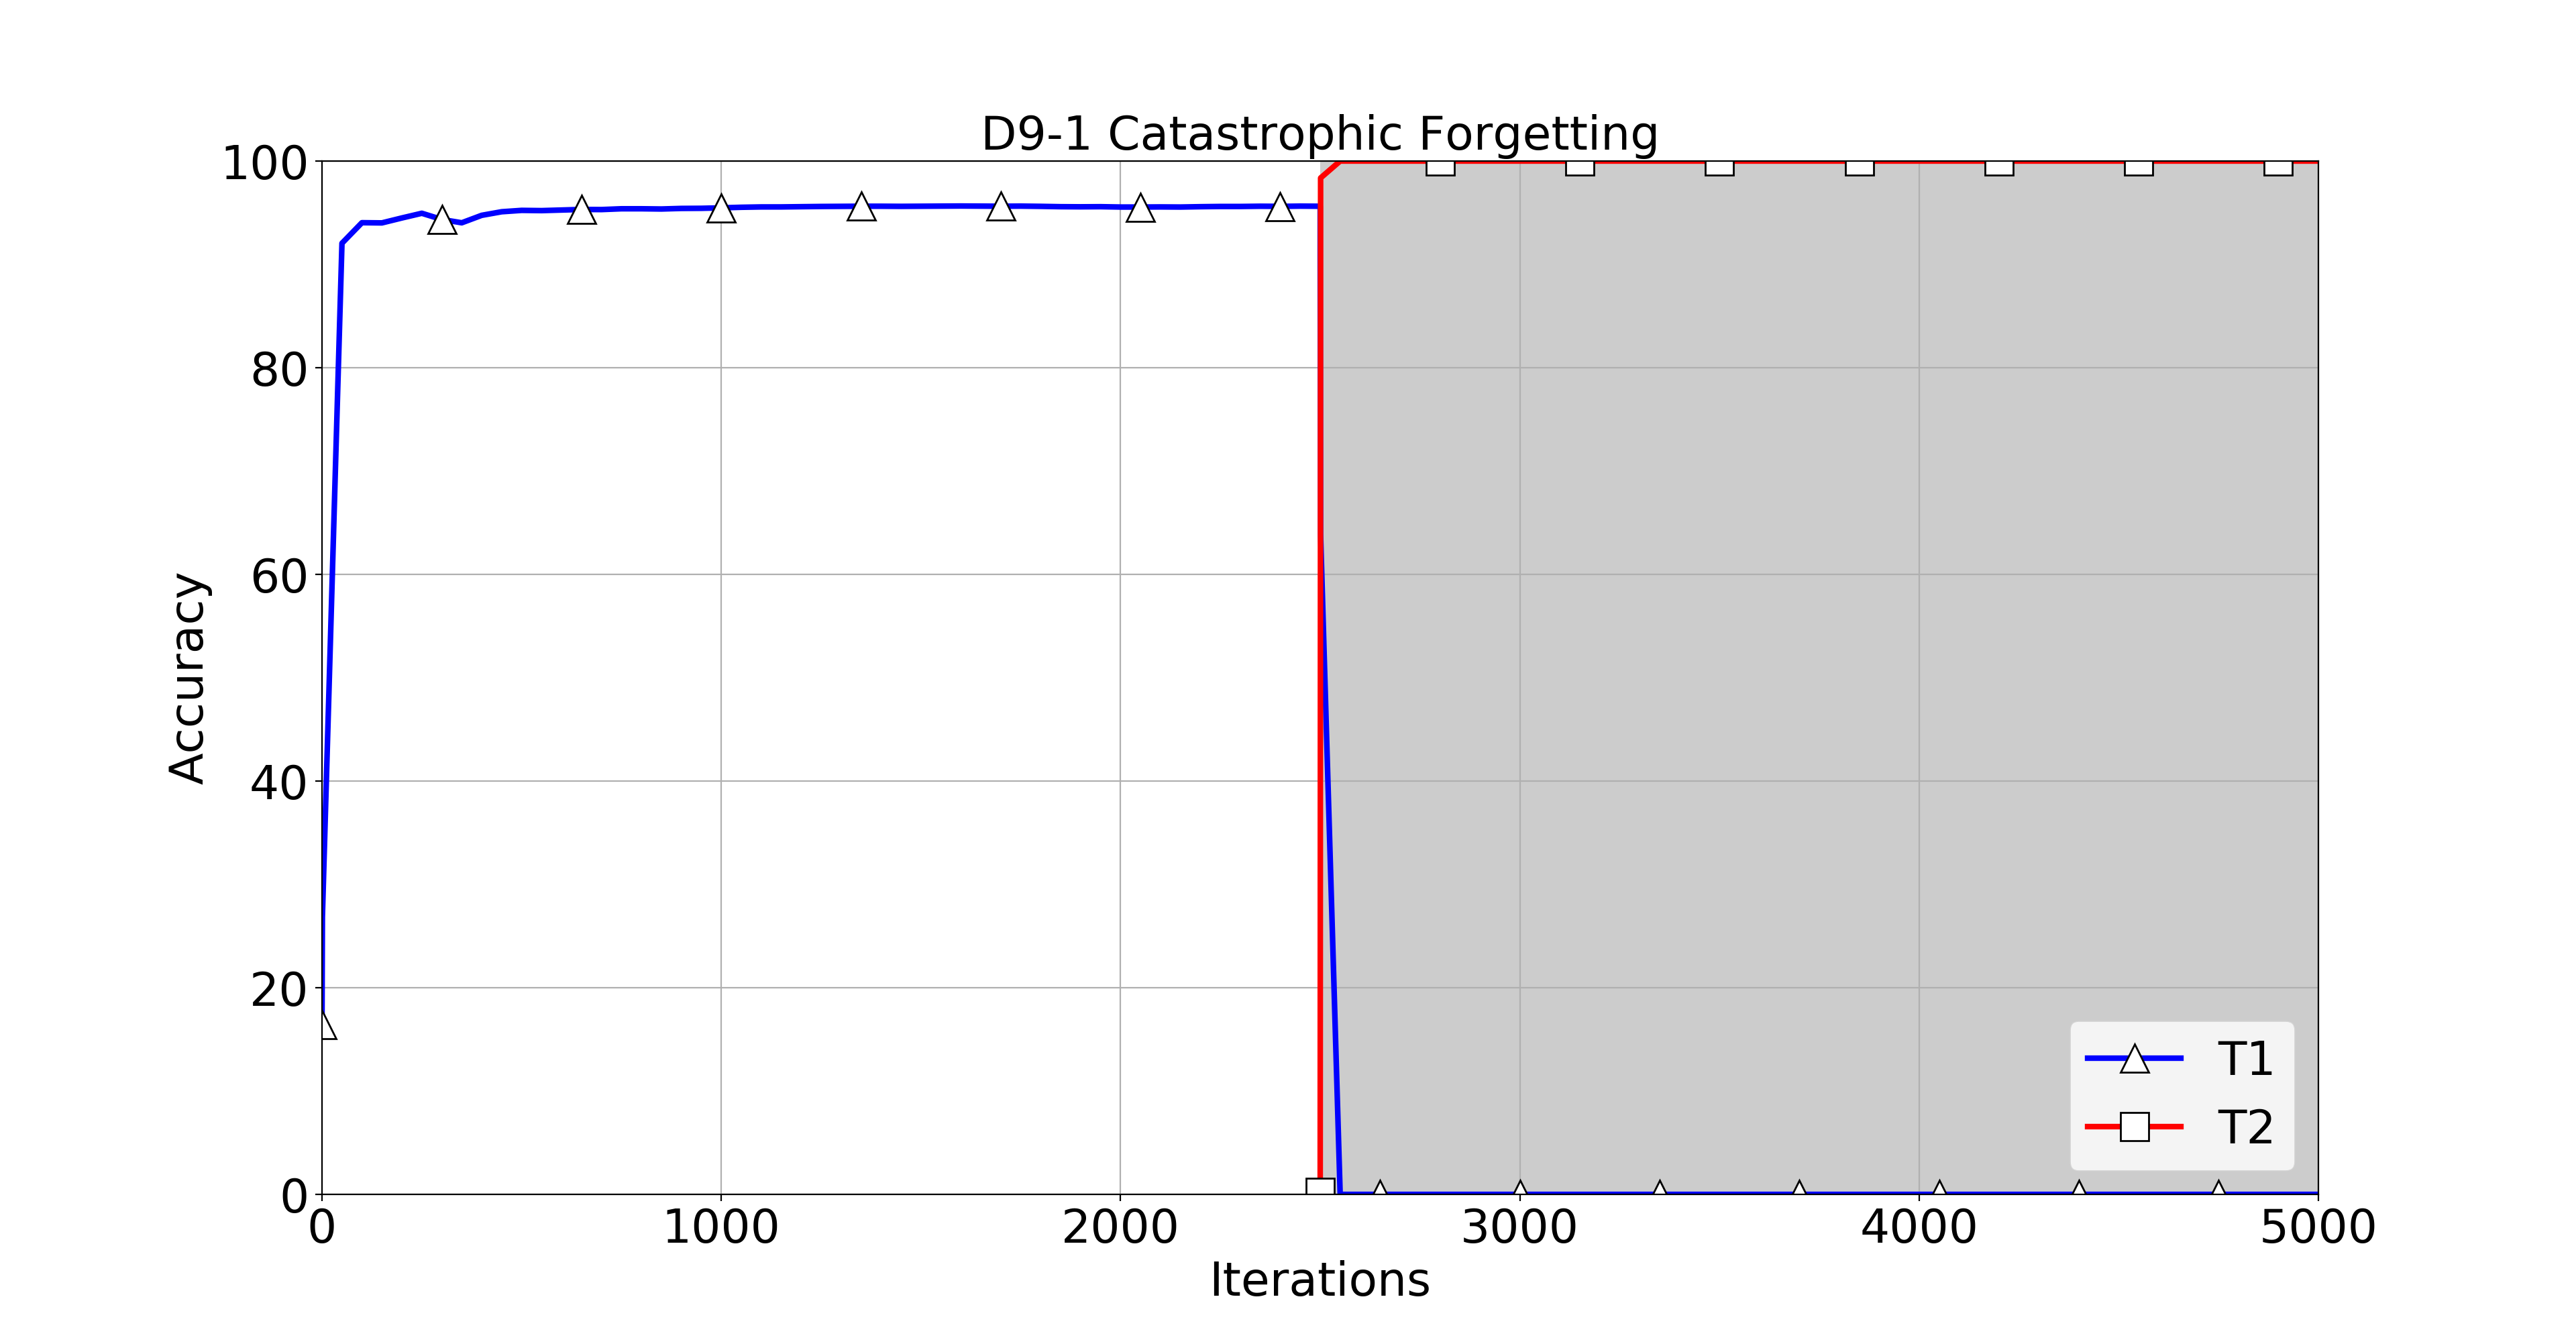
\includegraphics[width=\textwidth]{D91_catastrophic_forgetting}
    \caption{Catastrophic forgetting D9-1 example}
    \label{fig:catastrophic_forgetting_d91_example}
\end{figure}

Figure \ref{fig:catastrophic_forgetting_d91_example} shows the D9-1 benchmark.
After the training, $T_1$ results in 96\% accurcay.
With the start of the re-training, the accuracy of $T_1$ drops immediately.
$T_2$ on the other side gets quick results.
\newline
The immidiate drop of knowledge is represented by catastrophic forgetting.

\begin{figure}[H]
    \centering
    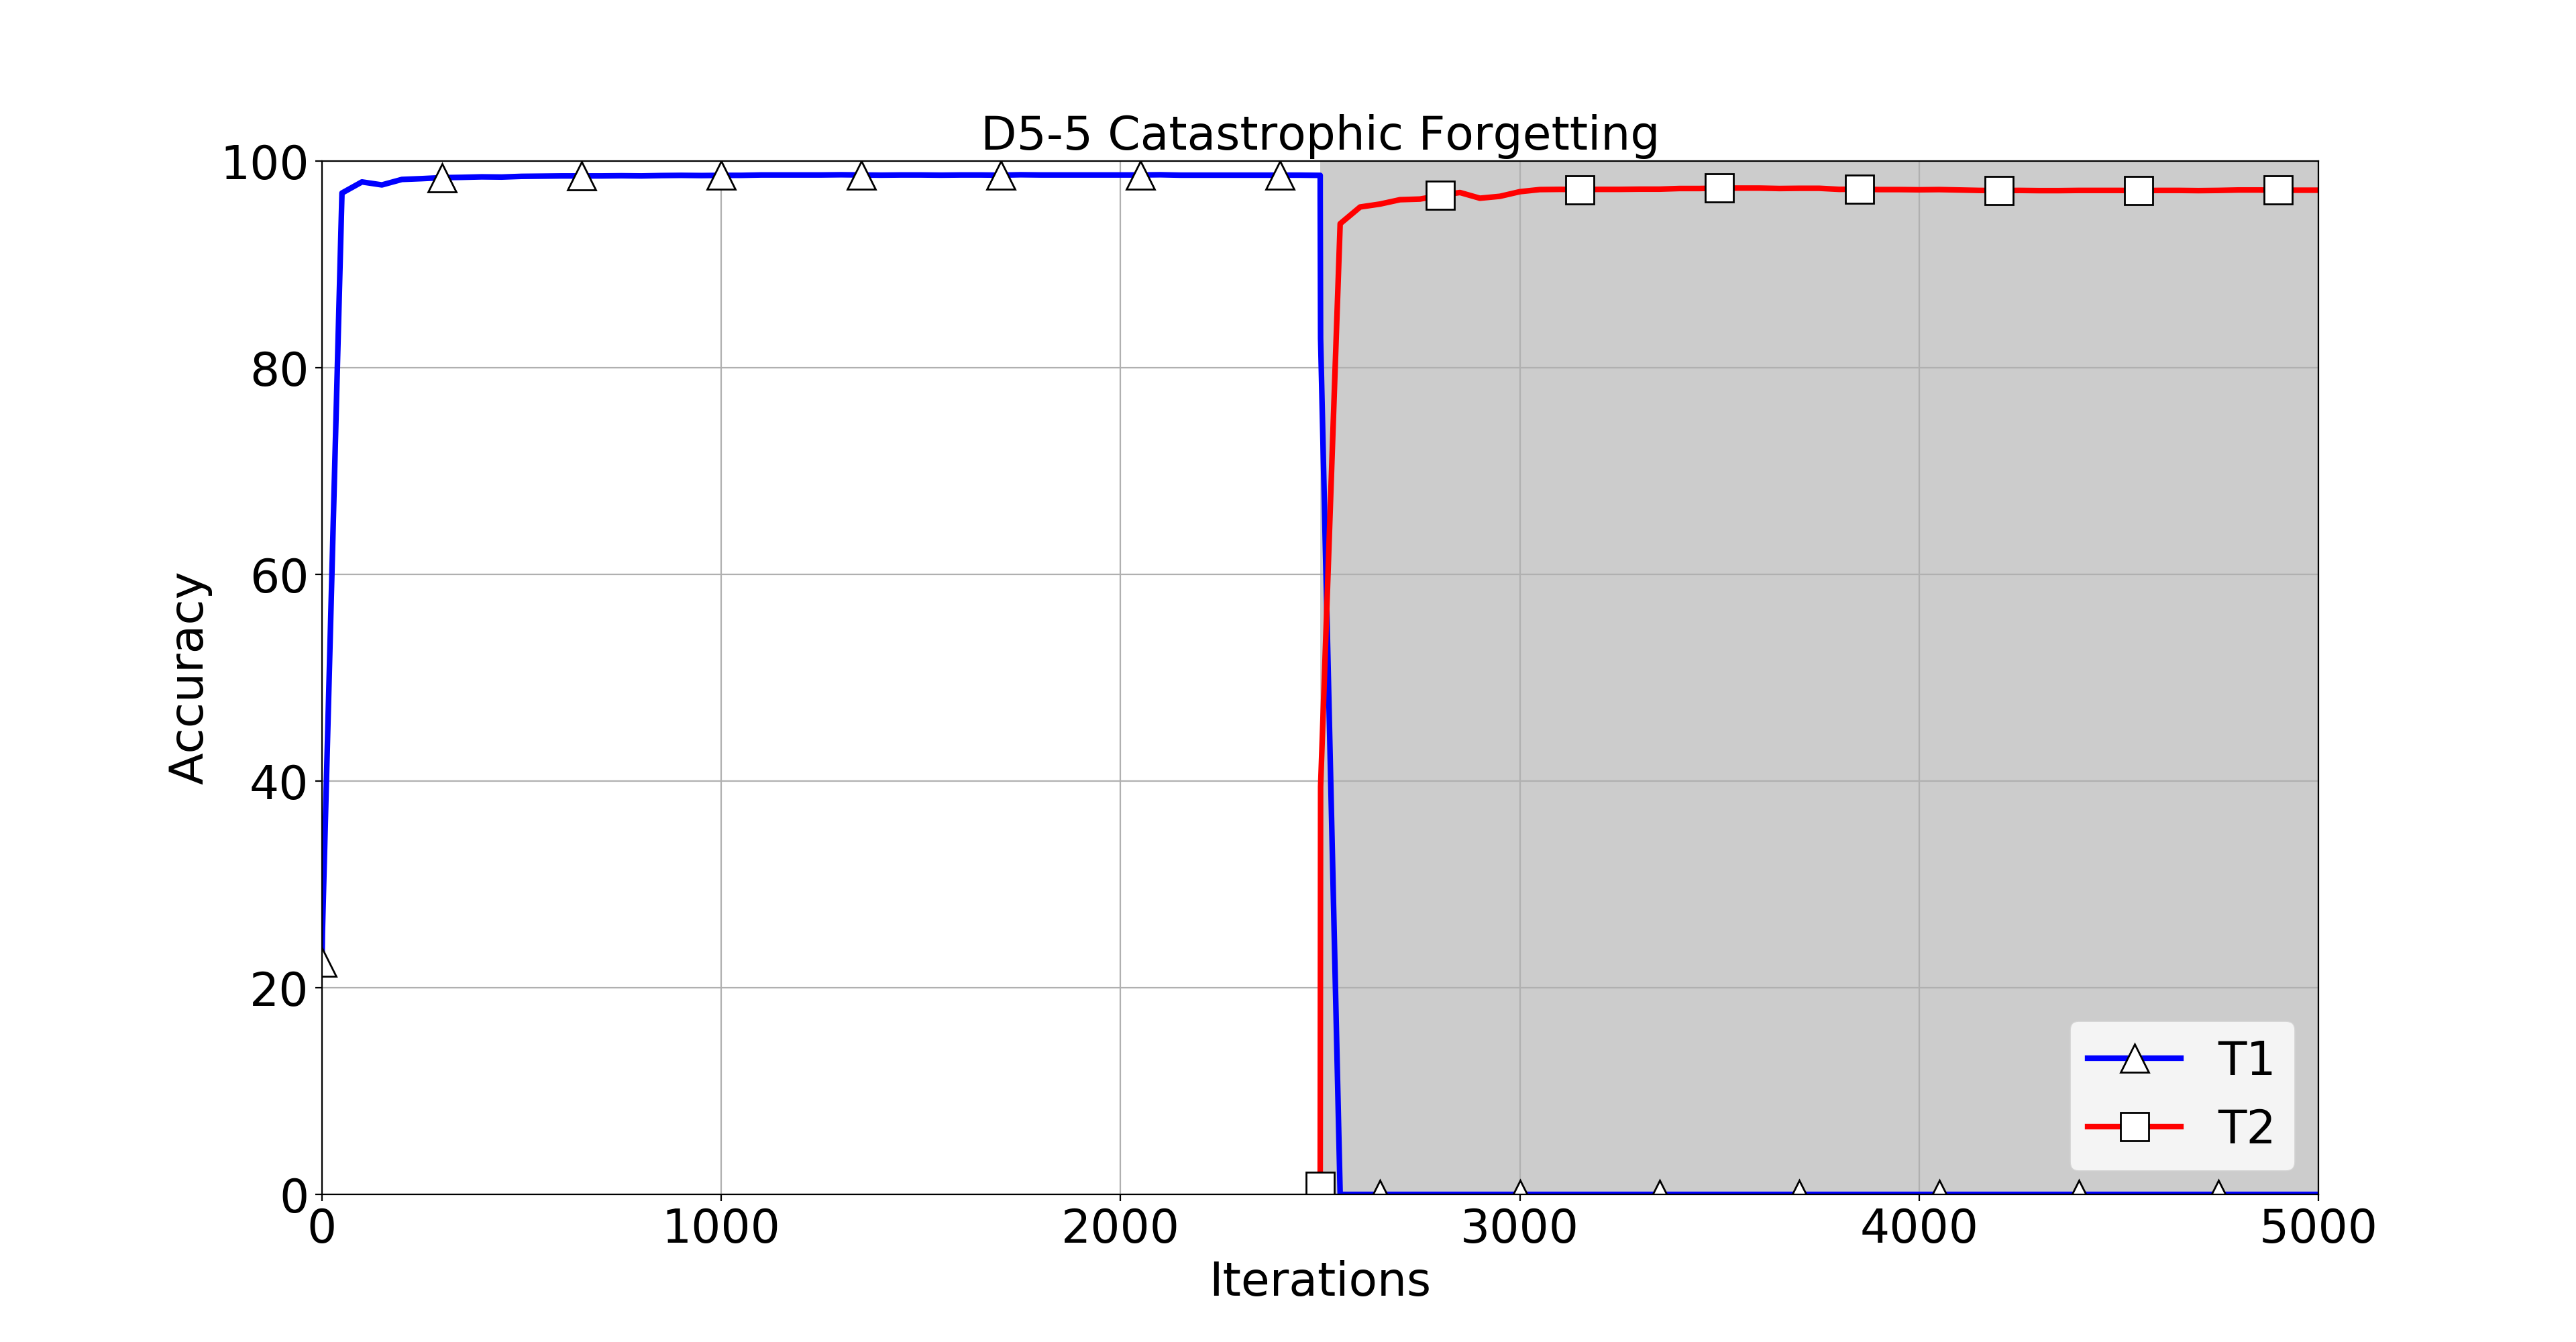
\includegraphics[width=\textwidth]{D55_catastrophic_forgetting}
    \caption{Catastrophic forgetting D5-5 example}
    \label{fig:catastrophic_forgetting_d55_example}
\end{figure}

Figure \ref{fig:catastrophic_forgetting_d55_example} shows the D5-5 benchmark.
As well as in Figure \ref{fig:catastrophic_forgetting_d91_example} the catastrophic forgetting happens immediately after the start of the re-training.

Catastrophic forgetting was first discovered by McCloskey and Cohen in 1989.
They documented their research in the article "Catastrophic Intereference" \cite{psychology_learning_mccloskey_cohen} and explained the problem in a rather simplified version:
\cite{psychology_learning_mccloskey_cohen}
\newline
Figure \ref{fig:catastrophic_forgetting_clarification} shows a propositional network representing artithmetic facts.
The network structure and connections in Figure \ref{fig:catastrophic_forgetting_clarification}A represent two facts, $5 + 4 = 9$ and $6 + 4 = 10$.
The learning of a new fact involves an extension to the current propositional structure.
Figure \ref{fig:catastrophic_forgetting_clarification}B shows the expansion of the fact $7 + 4 = 11$.
The seperation of each fact does not disrupt any knowledge.
\cite{psychology_learning_mccloskey_cohen}
\newline
Neural networks on the other hand are quite different.
Each connection and node responses to many different inputs.
In order to gain new knowledge, the neural network requires a change of the connection values (weights) and neuron values (bias).
Thus, this adjustement of the structure results in forgetting the previously acquired knowledge.
\cite{psychology_learning_mccloskey_cohen}

\begin{figure}[H]
    \centering
    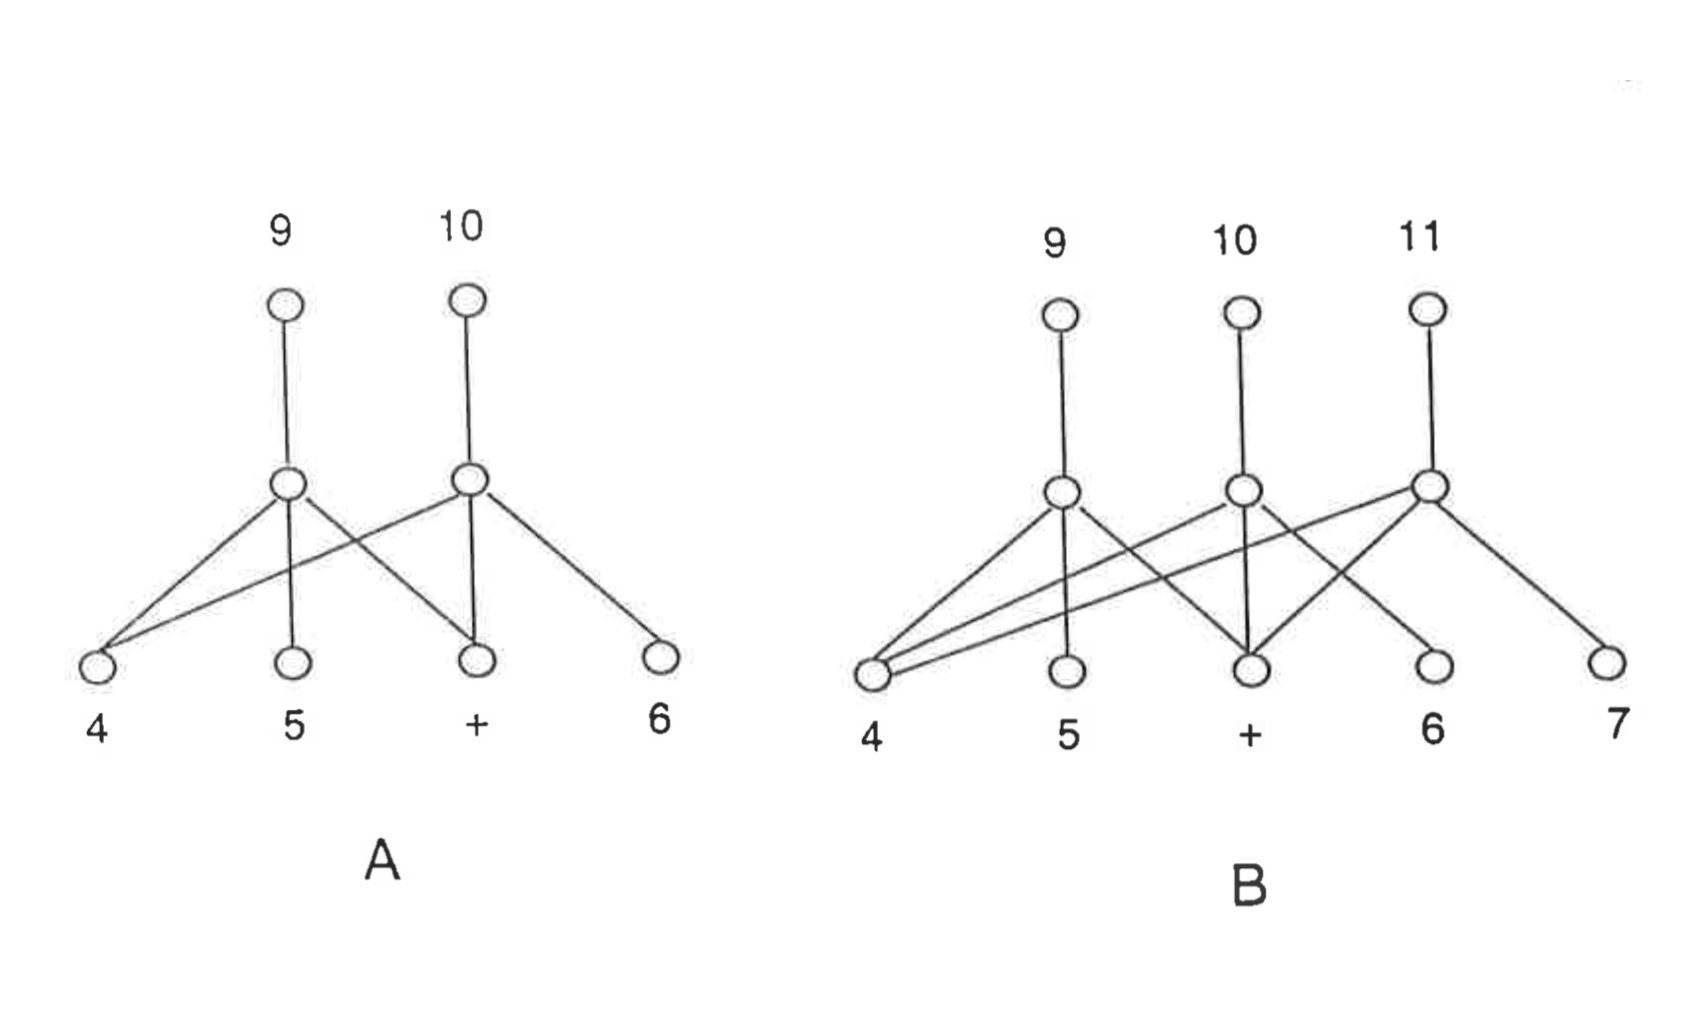
\includegraphics[width=\textwidth]{McCloskeyCohen1989CatastropicInterference}
    \caption{\cite[page 148]{psychology_learning_mccloskey_cohen} Catastrophic forgetting clarification}
    \label{fig:catastrophic_forgetting_clarification}
\end{figure}

\section{Elastic Weight Consolidation}
\label{foundation_ewc}

In order to overcome this catastrophic forgetting or at least reduce it, a team of researchers published a white paper called "Overcoming catastrophic forgetting" in 2016.
\cite{elastic-weight-consolidation}

At first they analysed the human brain as well as animal brains.
Here, they discovered that the mammalian brain may avoid catastrophic forgetting by protecting previously-acquired knowledge.
They developed an algorithm for deep neural networks and called it Elastic Weight Consolidation.
By showing tests in supervised learning and reinforcement learning, several tasks could sequentially trained without forgetting older ones.
\cite{elastic-weight-consolidation}

According to their paper, many configurations of $\theta$ (set of weights and biases) will result in the same performance of the network.
An over-parameterization of $\theta$ enables to find a solution for the next task, where the parameters are close to the previous task.
While learning the next task, \acrshort{ewc} wants to protect the performance of the previous task by limiting the parameters.
They should stay in a given region for a low error.
\cite{elastic-weight-consolidation}

In order to determine which values are most important, they see the training from a probabilistic perspective.
Here, they discovered that the catastrophic forgetting does not happen in a fully Bayesian way.
\cite{elastic-weight-consolidation}

% TODO Bayes inference

The Bayes theorem describes the probability of an event, based on prior knowledge of conditions that might be related to the event \cite{Bayes_theorem}. \cite{elastic-weight-consolidation, schaeffer_ewc}
\newline
The dataset $\mathcal{D}$ with included samples is given.
The network has to find the likelihood of the parameters (weights and biases) in $\theta$ given that $\mathcal{D}$ is occured.
This conditional probability $p \left(\theta | \mathcal{D} \right)$ is calculated by using the Bayes' rule: \cite{elastic-weight-consolidation, schaeffer_ewc}

\begin{equation}
    p \left( \theta | \mathcal{D} \right) = \frac{p \left(\mathcal{D}|\theta\right) p\left(\theta\right)}{p \left( \mathcal{D} \right)}
\end{equation}

$p \left( \theta \right)$ and $p \left( \mathcal{D} \right)$ are marginal probabilities. These are the probabilities for each event independently.
\newline
If the log-transform gets applied, the equation writes as follows: \cite{elastic-weight-consolidation, schaeffer_ewc}

\begin{equation}
    \setlength{\jot}{5pt}
    \begin{split}
        \log p(\theta | \mathcal{D}) & = \log \left[ 
                \frac{p \left(\mathcal{D}|\theta\right) p\left(\theta\right)}{p \left( \mathcal{D} \right)} 
            \right]
        \\
        & = \log p(\mathcal{D} | \theta) + \log p(\theta) - \log p(\mathcal{D})
    \end{split}
    \label{eq:bayes_applied_log}
\end{equation}

The paper assumes now that the data is split into two independent parts. $\mathcal{D}_A$ for task A and data $\mathcal{D}_B$ for task B.
This would work with more than two tasks, but for simplicity only two are used.
The re-arragne of the equation is: \cite{elastic-weight-consolidation, schaeffer_ewc}

\begin{equation}
    \setlength{\jot}{5pt}
    \begin{split}
        \log p(\theta | \mathcal{D}) 
        & = \log \big[
                p(\mathcal{D}_A | \theta) p(\mathcal{D}_B | \theta)
                \big]
            + \log p(\theta)
            - \log \big[
                p(\mathcal{D}_A) p(\mathcal{D}_B) 
             \big]
        \\
        & = \log p(\mathcal{D}_B | \theta)
            + \log p(\mathcal{D}_A | \theta)
            + \log p(\theta)
            - \log p(\mathcal{D}_A)
            - \log p(\mathcal{D}_B)
        \\
        & = \log p(\mathcal{D}_B | \theta)
            - \log p(\mathcal{D}_B)
            + \big[
                \log p(\mathcal{D}_A | \theta)
                + \log p(\theta)
                - \log p(\mathcal{D}_A)
                \big]
    \end{split}
\end{equation}

This last rearragement is almost similar to the Formula \eqref{eq:bayes_applied_log}.
Only $\mathcal{D}_A$ is replaced by $\mathcal{D}$.
Since they are equivalent to the conditional probability of the network's parameters given taskA's data, the equation can be modified to: \cite{elastic-weight-consolidation, schaeffer_ewc}

\begin{equation}
    \log p(\theta | \mathcal{D})=
       \log p(\mathcal{D}_B | \theta)
     + \log p(\theta | \mathcal{D}_A)
     - \log p(\mathcal{D}_B)
    \label{eq:bayesian_modified}
\end{equation}

Interesting on this formula is, that it still calculates the entire dataset (left side of Formula \eqref{eq:bayesian_modified}). Moreover, the paper descibes, that the right hand side only depends on the loss function for task B $\log p(\mathcal{D}_B | \theta)$. All information about task A is absorbed into the conditional probability $\log p(\theta | \mathcal{D}_A)$, the posterior distribution.
The paper follows that this conditional probability contains information about which parameters are important in solving task A.
\cite{elastic-weight-consolidation, schaeffer_ewc}
\newline
They state, that the true posterior distribution is intractable and follows with the Laplace approximation to approximate the posterior as a Gaussian distribution with mean given by the parameters of the previous task A and the diagonal precision by the diagonal of the Fisher information matrix.
\cite{elastic-weight-consolidation}
\newline
Furthermore, they inform that the Fisher information matrix is equivalent to the second derivative of the loss near a minimum and that "…it can be computed from first-order derivatives alone and is thus easy to calculate even for large models…" \cite{elastic-weight-consolidation} and "…it is guaranteed to be positive semi-definite."
\cite{elastic-weight-consolidation}.
\cite{elastic-weight-consolidation, schaeffer_ewc}
\newline
As a result they propose the new loss function for the upcoming training of task B:

\begin{equation}
    \mathcal{L}(\theta) = \mathcal{L}^{CE}(\theta) + \sum_{i} \frac{\lambda}{2} F_{i} (\theta_{i} - \theta_{A,i}^{*})^2
\end{equation}

The loss $\mathcal{L}(\theta)$ for task B consists of the originial loss $\mathcal{L}^{CE}(\theta)$ and the \acrshort{ewc} appendix.
Lambda ($\lambda$) in the \acrshort{ewc} appendix is a factor that determines how important the old task is compared to the new one \cite{elastic-weight-consolidation}.
The parameter $i$ is the iterator for each parameter (weights and biases) of the matrices.
The parameter F is the Fisher information matrix, which looks like this \cite{incremental-moment-matching}:

\begin{equation}
    F_{ij} = \frac{1}{N} \sum_{n=1}^{N} \frac{\partial \mathcal{L} \left( x_n \right) }{\partial \theta_{i}} \cdot \frac{\partial \mathcal{L} \left( x_n \right) }{\partial \theta_{j}}
\end{equation}

N represents all training samples, $\mathcal{L}$ the loss function and $\theta$ the set of all weights and biases.
In the paper the authors show some results with their algorithm on three different tasks with supervised learning. Figure \ref{fig:ewc_permuted_example} shows three permuted MNIST tasks:
\begin{figure}[H]
    \centering
    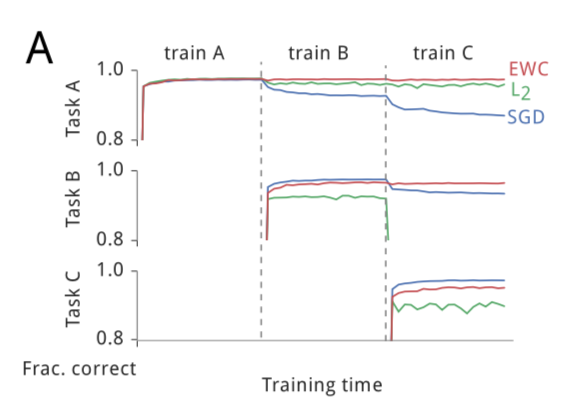
\includegraphics[scale=.5]{ewc_permuted_example}
    \caption{\cite{elastic-weight-consolidation} Original EWC results on permuted MNIST}
    \label{fig:ewc_permuted_example}
\end{figure}